\documentclass{bilidoc}

\geometry{
  a4paper,%
  left = 1.5cm,%
  right = 1.5cm,%
  top = 2.0cm,%
  bottom = 2.0cm%
}%



\usepackage{ulem}

\title{\textbf{\href{https://ascelibrary.org/doi/10.1061/(ASCE)GT.1943-5606.0002314}{Data Compilation from Large Drained Compression Triaxial Tests on Coarse Crushable Rockfill Materials \\粗碎石料的大型排水三轴压缩试验数据汇编}}}

\author{Carlos Ovalle \thanks{
    Assistant Professor, Dept. of Civil, Geological and Mining Engineering, Polytechnique Montreal, 2900 Edouard Montpetit Blvd., Montreal, QC, Canada H3T1J4; Research Institute of Mining and Environment, RIME UQAT-Polytechnique, 2900 Edouard Montpetit Blvd., Montreal, QC, Canada H3T1J4 (corresponding author). ORCID: \url{https://orcid.org/000-0002-9648-5262}. Email: \url{carlos.ovalle@polymtl.ca}.
} \and Sandra Linero \thanks{
    Principal Geotechnical Engineer, SRK Consulting (Australasia) Pty Ltd., Level 17, 44 Market St., Sydney, NSW 2000, Australia.
} \and Christophe Dano \thanks{
    Associate Professor, Centre National de la Recherche Scientifique, Institut National Polytechnique, Univ. Grenoble–Alpes, 3SR, 1270 rue de la piscine, Domaine Universitaire, Grenoble 38000, France.
} \and Edgar Bard \thanks{
    Senior Mine Waste Consultant, Golder Associates, 181 Magdalena, Las Condes 7550055, Chile.
} \and Pierre-Yves Hicher \thanks{
    Emeritus Professor, Centre National de la Recherche Scientifique, Unité Mixte de Recherche, Ecole Centrale de Nantes, 1 Rue de la Noë, Nantes 44300, France. 
}\and Rodrigo Osses \thanks{
    Ph.D. Candidate, Dept. of Structural and Geotechnical Engineering, Pontificia Universidad Cat´olica de Chile, 4860 Av. Vicu˜na Mackenna, Macul 7820436, Chile; Facultad de Ingeniería y Ciencias, Departamento de Ingeniería de Obras Civiles, Universidad de La Frontera, 1145 Francisco Salazar, Temuco 4811230, Chile.
} \thanks{
    Note. This manuscript was submitted on August 30, 2019; approved on March 18, 2020; published online on June 27, 2020. Discussion period open until November 27, 2020; separate discussions must be submitted for individual papers. This technical note is part of the {\em\bfseries Journal of Geotechnical and Geoenvironmental Engineering}, © ASCE, ISSN 1090-0241.
}}

\date{}

\begin{document}

\maketitle

\vspace{-7mm}

\begin{Abstract}{Rockfill; Large triaxial tests; Particle crushing; Shear strength; Secant stiffness.}{碎石;大型三轴试验;颗粒破碎;剪切强度;割线刚度。}

    Investigating the mechanical properties of rockfills requires laborious, time-consuming, and expensive large-scale testing. Therefore, practitioners frequently adopt design parameters based on a limited number of reports with experimental results. With the aim of enlarging and consolidating the database on the mechanical behavior of coarse rockfills, this paper compiles 158 drained triaxial compression tests conducted on 33 different materials, performed on samples∼1 m in diameter and having a maximum particle size between 100and 200mm. Data are analyzed in terms of particle breakage, shear strength, and stiffness. The results are compared with limits for high and low shear strength previously reported. At confining pressures lower than 0.2 MPa, rockfills consistently have a maximum internal friction angle higher than 45°; at high pressure, this value decreases to a range between 30° and 40°, mainly due to degradation caused by particle breakage. Average secant Young’s moduli for all uniform and well-graded rockfills analyzed are in the typical range for loose sands, characterized by a normalized secant modulus of 100 to 200. 

    \switchcolumn

    研究碎石的机械性能一般需要费力,费时且昂贵的大规模试验。 因此,从业人员经常根据数量有限的报告和实验结果选用设计参数。为了扩大和巩固有关粗碎石料力学性能的数据库,本文汇编了对33种不同材料进行的158次排水三轴压缩试验,这些试验的样本直径约为1米,其最大粒径在100到200毫米之间。然后我们根据颗粒破损程度,剪切强度和刚度来分析试验数据。将结果与先前报道的高和低剪切强度极限进行比较。 在围压低于0.2MPa的情况下,碎石料的最大内摩擦角始终大于45°。在高压下,该值减小到30°至40°之间,这主要是由于颗粒破裂引起的土块降解。对于所有分析的均匀且分级良好的碎石料,平均正割杨氏模量都在松散砂体的典型范围内,其特征是正割杨氏模量在100到200之间。
    
\end{Abstract}

\begin{ParaColumn}[\bisection*{Introduction}{介绍}]

    Owing to their massive production potential by quarrying and their mechanical properties in the dense state, rockfills are frequently used in civil engineering works. These granular fills are mainly composed of a mix of sand and angular rock aggregates with oversized particles that are too large to be handled by standard laboratory devices for compression and shearing. Alternative laboratory and in situ large direct shear tests have been developed by others \citep{Barton1981873,Matsuoka200192,Estaire200673}. However, these methodologies only allow for the evaluation of the mechanical behavior at low stresses, while calibration of new constitutive models that have been specifically developed for rockfill behavior \citep{Chávez2003215,Varadarajan2003206,Xiao20171,Yin2017} require accurate data on stress-strain controlled response over a large range of stresses. Therefore, a common challenge that engineers face when designing rockfill structures is that published information which documents large-scale tests is very scarce.

    \switchcolumn

    由于其巨大的采石生产潜力和致密状态下的机械性能,碎石经常用于土木工程。 这些颗粒状填充物主要由砂和角砾石骨料与超大颗粒的混合物组成,由于颗粒太大,无法通过标准实验室设备进行压缩和剪切处理。 有人已经开发了替代的实验室和现场大型直接剪切试验\citep{Barton1981873,Matsuoka200192,Estaire200673}。 但是,这些方法仅可用于评估低应力下的力学行为,而新的校准本构模型\citep{Chávez2003215,Varadarajan2003206,Xiao20171,Yin2017}是专门为碎石力学行为开发的,这需要在大范围的应力应变控制下的响应的准确数据。因此,工程师在设计碎石结构时面临的共同挑战是,记录大规模试验的公开信息非常稀缺。

    \switchcolumn*

    The largest triaxial testing apparatus ever built handles specimens with a diameter of ∼1 m. While equipment of this scale has been built, there are few examples currently in use due to the high cost involved in their maintenance and operation. Pioneering development of testing on very large samples was first reported during the 1960s at the laboratories of Karlsruhe Technical University \citep{Leussink1960}, the University of California at Berkeley (UCB) \citep{Marachi1969}, and the Federal Electricity Commission of Mexico (CFE) \citep{Marsal1965}. These groups designed and built devices that could handle samples ranging in diameter ($D$) from 914 to 1,130 mm, and having a maximum particle size (dmax) of 200 mm using the classic minimum aspect ratio $D/d_{\max}=$ 5 to 6 \citep{Holtz19561}. Experimental programs at CFE and UCB were carried out on several rockfill dam materials, and the results have become a reference for engineers and researchers. Part of the data produced at the CFE and UCB laboratories has been analyzed in detail and used to propose empirical correlations and ranges for mechanical parameters of coarse rockfill materials \citep{Leps19701159,Barton1981873,Hunter2003909}. Other authors have subsequently reported new results and have updated the database \citep{Charles1980353,Al-Hussaini1983706,Matsuoka1998275,Hunter2003909,Varadarajan2003206,Xiao2014a,Xiao2014b} using triaxial cells that can take samples of 300–500 mm in diameter. These studies have significantly advanced the understanding of the mechanical behavior of rockfills, such as the study of the effects of partial saturation \citep{Oldecop2003289,Alonso2016455}, stress path \citep{Chávez2003215,Xiao2016}, and particle size \citep{Verdugo2007243,Hu2011,Ovalle20201}.

    \switchcolumn

    历史上最大的三轴试验设备可处理直径约1米的样本。 虽然这种规模的设备已经可以制造,但是由于维护和操作成本高昂,目前很少使用这些设备。  1960年代,卡尔斯鲁厄技术大学\citep{Leussink1960},加利福尼亚大学伯克利分校(UCB)\citep{Marachi1969}和墨西哥联邦电力委员会的实验室(CFE)\citep{Marsal1965}首次报道了对大型样品进行试验的开创性发展。这些小组设计和制造了可以处理直径($D$)从914到1130毫米范围的样品,并且使用经典的最小长宽比$D/d_{\max}=5\sim 6$ \citep{Holtz19561}。 CFE和UCB的试验程序是在几种碎石坝材料上进行的,其结果已成为工程师和研究人员的参考。 许多人对CFE和UCB实验室得到的部分数据进行了详细分析,并用于提出经验性的相关性和取值范围范围,用作粗碎石料的力学参数\citep{Leps19701159,Barton1981873,Hunter2003909}。 其他作者随后使用可以采集直径为300-500毫米的土体样品的三轴试验报告了新的结果并更新了数据库\citep{Charles1980353,Al-Hussaini1983706,Matsuoka1998275,Hunter2003909,Varadarajan2003206,Xiao2014a,Xiao2014b}。 这些研究极大地促进了对碎石力学行为的理解,例如对部分饱和度的影响\citep{Oldecop2003289,Alonso2016455},对应力路径\citep{Chávez2003215,Xiao2016}和对颗粒粒径\citep{Verdugo2007243,Hu2011,Ovalle20201}的研究。

    \switchcolumn*

    Due to the size limitation of testing devices, a common practice is to test small-scale samples with a parallel gradation while maintaining the particle shape, mineralogy, and sample aspect ratio. However, it has been proven that this method may be limited due to size effects on particle crushing \citep{Marachi1969,Frossard2012415,Ovalle20142199}. \enautoref{figure:1} presents the results of several diametral compressions of individual rock aggregates between two stiff parallel platens where crushing strength decreases when particle size increases, which is consistent with the brittle fracture mechanics theory \citep{Weibull19391}. Therefore, the amount of particle crushing is less in small-scale (i.e., finer) granular materials than in coarser prototype materials.

    \switchcolumn

    由于试验设备的尺寸限制,通常的做法是在保持颗粒形状,矿物质和样品长宽比不变的同时,对小尺度样品进行平行试验。 但是,已经有人证明该方法可能会由于尺寸上的影响而受到限制\citep{Marachi1969,Frossard2012415,Ovalle20142199}。 \cnautoref{figure:1}给出了两个刚性平行压板之间单个岩石聚集体的多次径向压缩的结果,其中,当粒径增大时,抗压强度降低,这与脆性断裂力学理论\citep{Weibull19391}一致。 因此,小颗粒物料的颗粒破碎量比粗颗粒物料的颗粒破碎量要小。

    \CrossColumnText{
        \begin{figure}[htb]
    \centering
    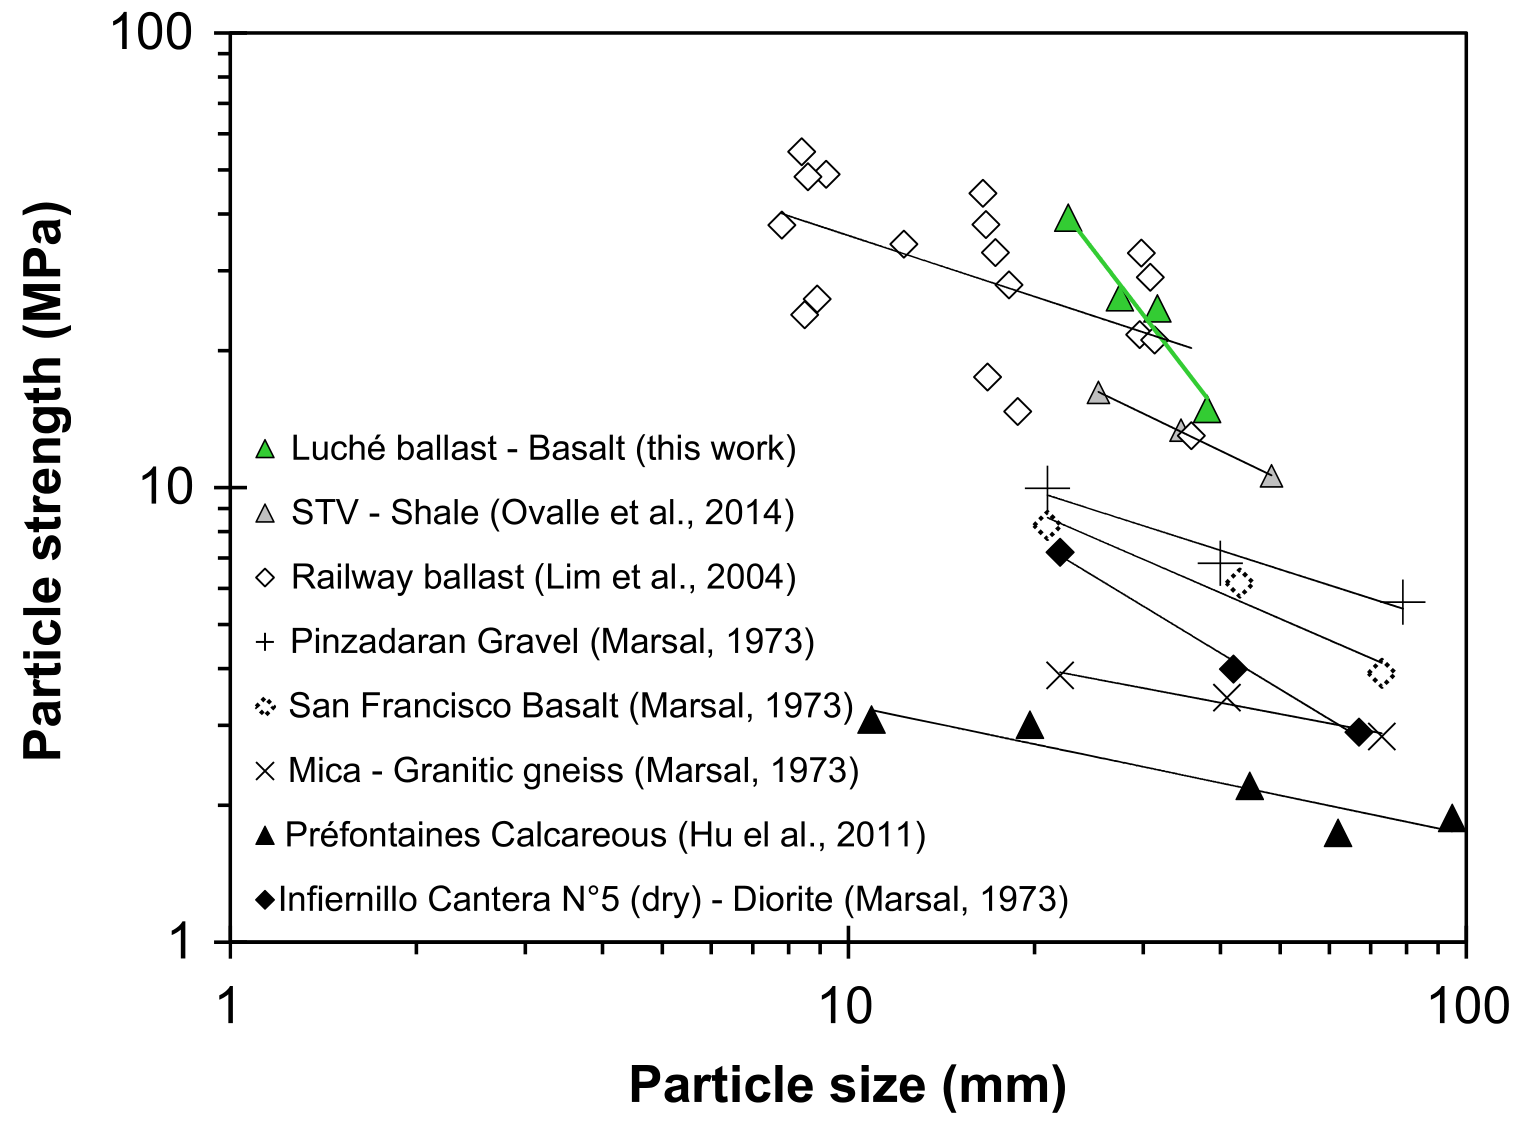
\includegraphics[width=0.5\textwidth]{figures/figure-1.png}
    \bicaption{Particle crushing strength of rock aggregates}{骨料的颗粒破碎强度}
    \label{figure:1}
\end{figure}
    }

    \switchcolumn*

    Along with presenting new tests carried out in recent, very large triaxial devices, the aim of this study was to consolidate and extend the existing database through the compilation of data on large triaxial tests on coarse rockfill samples carried out between the 1960s and the 2000s. To present comparable results in terms of stress path, particle size, and particle shape, only drained compression triaxial tests on coarse rockfills samples of $\sim 1$ m in diameter, composed of angular shaped grains with $d_{\max}$ between 100 and 200 mm, have been considered. Results from 158 tests on samples from 33 rockfill materials are presented. The influence of the confining stress and the amount of particle crushing on shear strength and secant stiffness is discussed. To highlight the data on coarse crushable rockfill materials, the results were compared with published data on finer materials, such as dense uniform quartzitic sands and railway ballasts.

    \switchcolumn

    除了介绍最近在非常大的三轴设备中进行的新试验外,本研究的目的是通过汇编有关在1960年代至2000年代之间进行的粗碎石料样品的大型三轴试验的数据来加强和扩展现有数据库。 为了在应力路径,粒度和颗粒形状方面提供可比的结果,仅考虑了对直径约1米的粗碎石样品进行的排水三轴试验,该样品由$d_{\max}$在100至200毫米之间的角状晶粒组成。 给出了158种试验结果,这些结果来自33种碎石材料的样品。 讨论了围压和颗粒破碎量对剪切强度和割线刚度的影响。 为了突出有关粗碎石料的数据,将结果与已发布的有关较细材料的数据进行了比较,如致密均匀的石英砂和铁道石渣。

\end{ParaColumn}
\begin{ParaColumn}[\bisection*{Recent Experimental Data Included in the Database}{数据库中包含的最新试验数据}]
    
    Recently, new large triaxial devices have been operating at École Centrale Nantes (ECN) in France and at the IDIEM laboratory in Chile. The large device at ECN can test samples that are 1,000 mm in diameter and 1,500 mm in height, at a maximum confining pressure of 1.5 MPa. The IDIEM large triaxial device can handle samples of 1,000 mm in diameter and 1,800 mm in height at confining pressures up to 3 MPa. Exhaustive descriptions and testing methodologies can be found in \citet{Hu2011} and \citet{Ovalle2013} for ECN, and in \citet{DelaHozAlvarez2007} for IDIEM.

    \switchcolumn

    最近,新的大型三轴设备已经在法国的南特中央大学(ECN)和智利的IDIEM实验室中投入使用。 ECN的大型设备可以在最大1.5MPa的围压下对直径1000毫米,高度1500毫米的样品进行试验。IDIEM的大型三轴设备可以在最大3MPa的围压下处理直径1000毫米,高度1800毫米的样品。对ECN和IDIEM的详细描述和试验方法可以在\citet{Hu2011}和\citet{Ovalle2013}以及\citet{DelaHozAlvarez2007}中找到。

    \CrossColumnText{
        \begin{figure}[htb]
    \centering
    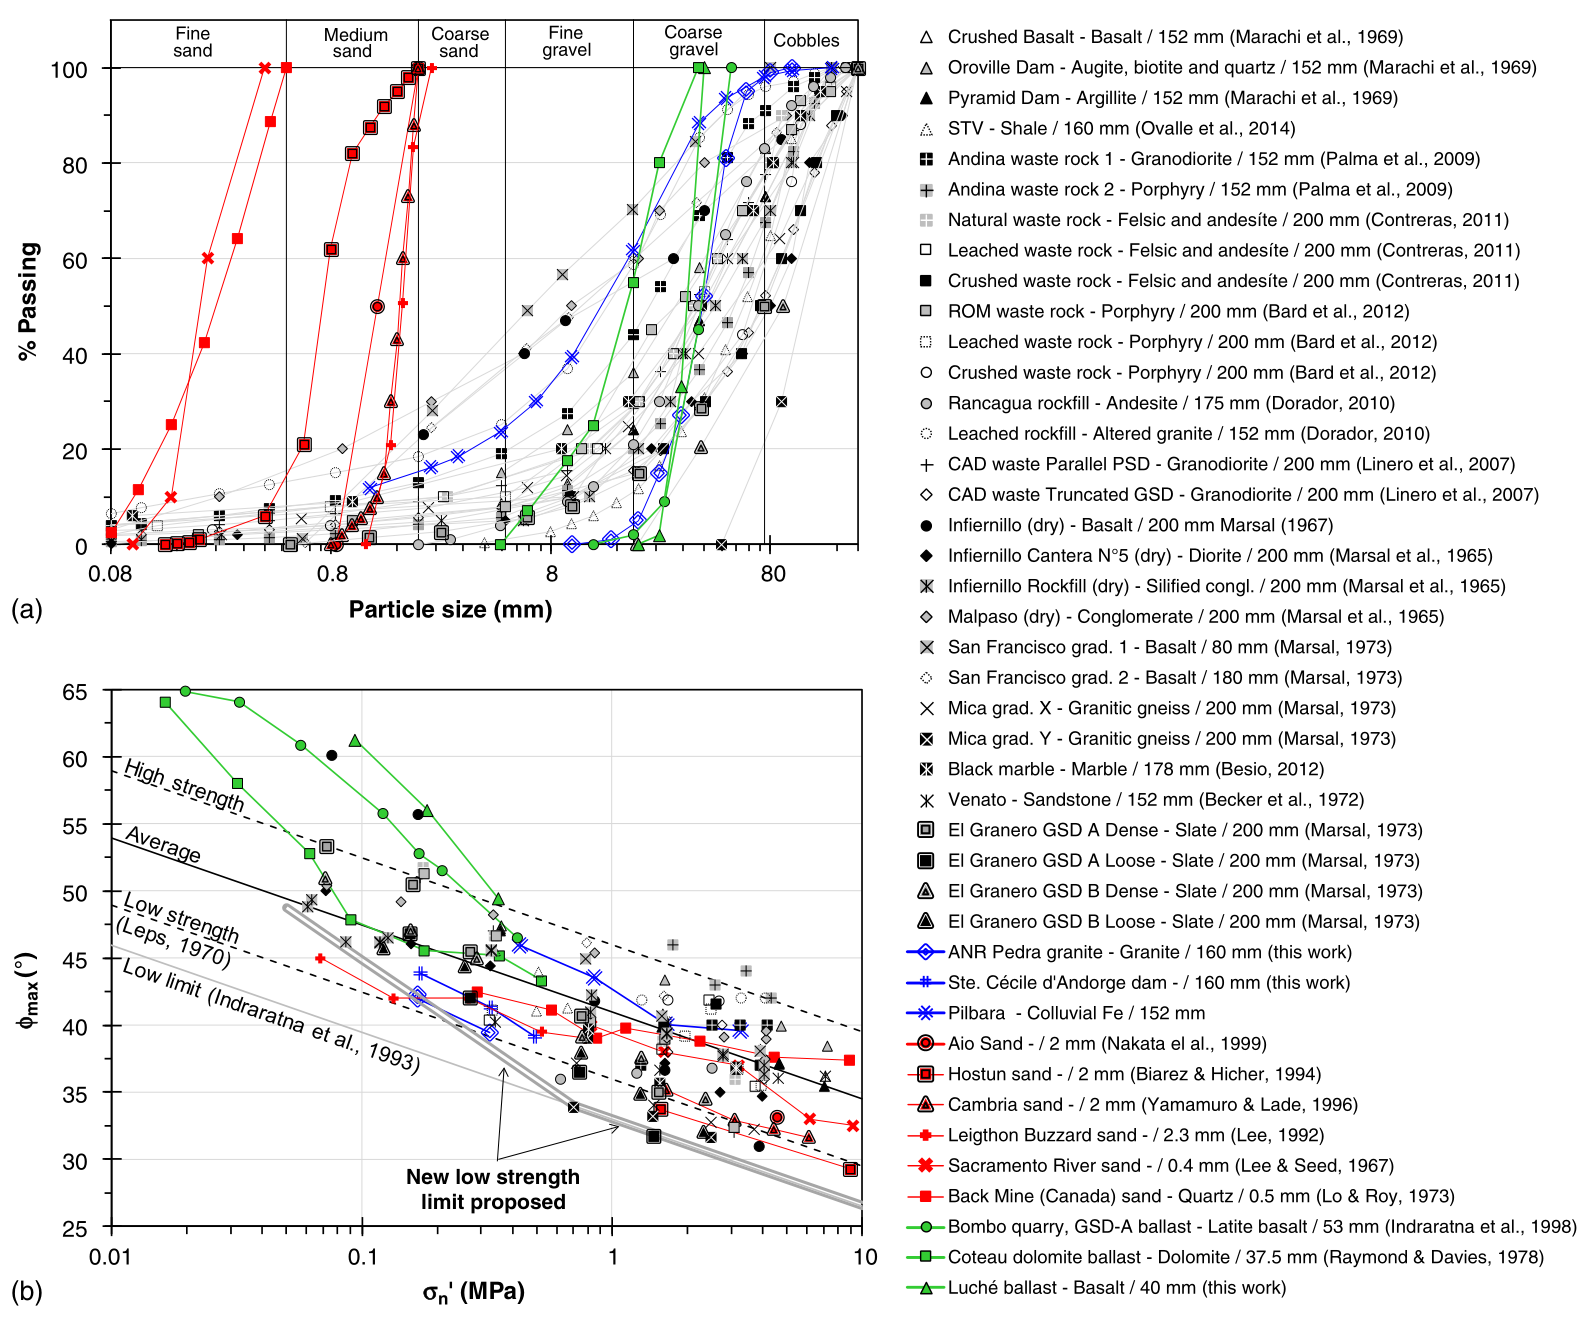
\includegraphics[width=\textwidth]{figures/figure-2.png}
    \bicaption{Compiled sands, ballasts, and rockfills: (a) GSD; and (b) maximum internal friction angle [legend: “Material Name/dmax (millimeters) (Ref.)”]}{汇编的砂土,铁道石渣和碎石料:(a)GSD; (b)最大内摩擦角[图例:“材料名称/$d_{\max}$(毫米)(参考)”]。}
    \label{figure:2}
\end{figure}
    }

    \switchcolumn*

    Among the 158 large triaxial tests on 33 materials compiled and analyzed, 14 rockfill materials were tested at IDIEM (1 unpublished — on Pilbara rockfill), 3 at ECN (2 unpublished — on Agence Nationale de la Recherche (ANR) Pedra granite and Sainte Cécile d’Andorge dam), 4 at UCB, and 12 at CFE. \enautoref{figure:2}(a) shows the grain size distribution (GSD) for each material. Descriptions of the new rockfills reported in this study are the following:

    \switchcolumn

    在已编制分析的33种材料的158个大型三轴试验中,有14种碎石料在IDIEM(1种未发表的Pilbara碎石)上进行了试验,3种在ECN(2种未发表的国家研究机构(ANR)花岗岩和圣塞西尔安道尔大坝),4种在UCB以及12种在CFE上分别进行了试验。 \cnautoref{figure:2}(a)显示了每种材料的颗粒尺寸分布(GSD)。 本研究报告的新碎石场描述如下:

    \switchcolumn*

    \begin{itemize}
        \item \textbf{Pilbara:} Waste crushed mining rockfill from the Pilbara region in Western Australia, consisting of Neogene alluvial and colluvial sediments originated from weathering, erosion, and transportation of Precambrian banded iron formation rocks.
        \item \textbf{ANR Pedra granite:} Washed, crushed angular granite rockfill.\\[-5mm]
        \item \textbf{Sainte Cécile d’Andorge dam:} Schist and mica-schist rockfill with subangular grains.
    \end{itemize}

    \switchcolumn

    \begin{itemize}
        \item \textbf{Pilbara:}来自西澳大利亚Pilbara地区的碎石矿山废碎石,由前寒武纪带状铁地层风化、侵蚀和搬运形成的新近纪冲积、冲积物组成。
        \item \textbf{ANR Pedra花岗岩:}洗碎的有棱角的花岗岩碎石。
        \item \textbf{Sainte Cécile d'Andorge大坝:}带有亚角粒的片岩和云母片岩。
    \end{itemize}

    \switchcolumn*

    The materials analyzed here have diverse origins, and differ in terms of relative density, mineralogy, particle shape, GSD, and water content (tests on saturated and air-dried samples). Accordingly, significant data scatter should be expected. However, due to the lack of available data to perform accurate analyses, this paper aims to present ranges of results for shear strength and secant Young’s modulus to compare the results with quartzitic sands and ballasts and to provide references for engineers and researchers. The analyses presented highlight the influence of the breakage ratio ($B_g$), using the definition of \citet{Marsal196727}, given by the sum of positive differences between the percentage of the total sample contained in each size fraction before and after the test.

    \switchcolumn

    此处分析的材料具有不同的来源,并且在相对密度,矿物成分,颗粒形状,GSD和含水量(在饱和和干燥的样品上进行试验)方面也不同。 因此,预期应该会有大量的数据分散。 但是,由于缺乏准确分析的数据,本文旨在介绍抗剪强度和割线杨氏模量的结果范围,以便与石英砂和铁道石渣进行比较,并为工程师和研究人员提供参考。 本文给出的分析使用\citet{Marsal196727}的定义强调了破损率($B_g$)的影响,该定义由试验前后各尺寸分数中所含总样品百分比的正差之和给出。

\end{ParaColumn}
\begin{ParaColumn}[\bisection*{Quartzitic Sands and Ballast Data Collected}{采集石英砂和石渣数据}]

    Compiled data from new tests on rockfills were compared with published data on dense uniform quartzitic sands and ballast materials, as well three new tests on Luché ballast. The results of drained triaxial compression tests with confining pressures over the same range as the database compiled for rockfill materials (e.g., from 1 to 10 MPa) were considered for the materials presented in \enautoref{table:1}; \enautoref{figure:2}(a) presents the GSD for each quartzitic sand and ballast.

    \switchcolumn

    将新的碎石场试验数据与已发布的关于致密的均匀石英砂和石渣材料的数据以及在Luché石渣上的三项新试验进行了比较。 对于\cnautoref{table:1}所示的材料,考虑了围压在与碎石材料数据库(例如1至10MPa)的数据库相同范围内的排水三轴压缩试验的结果;\cnautoref{figure:2}(a)给出了每种石英砂和石渣的GSD。

    \CrossColumnText{
        \begin{table}[htb]
    \centering
    \small
    \bicaption{Data collected on sands and ballast}{在砂土和石渣上收集的数据}
    \label{table:1}
    \tabcolsep=0.1mm
    \begin{tabular}{p{0.19\textwidth}<{\raggedright} p{0.27\textwidth}<{\raggedright} p{0.05\textwidth}<{\centering} p{0.12\textwidth}<{\centering} p{0.13\textwidth}<{\centering} p{0.23\textwidth}<{\raggedright}}
        \toprule
        Material & Description & $d_{\max}$ (mm) & LLA ($\%$) (for ballast only) & Relative density (for sands only) & Reference \\
        \midrule
        \multicolumn{6}{c}{Quartzitic sands} \\
        \midrule
        Hostun sand & 98$\%$ quartz angular & 2 & $-$ & 1 & \citet{Biarez19941} \\
        Aio sand& Quartz and 30$\%$ feldspar,  subrounded sand & 2 & $-$ & 1 & \citet{Nakata1999567} \\
        Cambria sand & Subrounded sand composed by a mix of quartz and gypsum & 2 & $-$ & 0.9 & \citet{Yamamuro1996109} \\
        Leighton Buzzard sand & Subrounded quartz sand & 2.3 & $-$ & 0.8 & \citet{Lee1992} \\
        Sacramento River sand & Subrounded quartz sand & 0.4 & $-$ & 1 & \citet{Lee1967117} \\
        Quartz sand & Angular, derived from crude quartz from Back mine, Canada & 0.5 & $-$ & 0.6 & \citet{Lo197361} \\
        \midrule
        \multicolumn{6}{c}{Railway ballast materials} \\
        \midrule
        Bombo ballast & Latite basalt from Bombo quarry, Australia & 53 & 15 & $-$ & \citet{Indraratna1998439} \\
        Coteau ballast & Dolomite from Coteau, Quebec, Canada & 37.5 & 17.6 & $-$ & \citet{Raymond1978737} \\
        Luché ballast & Diorite ballast from Luché quarry, France & 40 & 10 & $-$ & This work \\
        \bottomrule
    \end{tabular}
\end{table}
    }

\end{ParaColumn}
\begin{ParaColumn}[\bisection*{Analysis and Discussion}{分析与讨论}]

    \switchcolumn[0]*[\biparagraph{Shear Strength}{抗剪强度}]

    \enautoref{figure:2}(b) presents shear strength for all tests collected in terms of the maximum friction angle ($\phi_{\max}$) against the effective normal pressure on the failure plane ($\sigma_n^\prime$), according to the Mohr-Coulomb failure criterion. \enautoref{figure:2}(b) also includes the limits for high, average and low shear strength proposed by \citet{Leps19701159} and \citet{Indraratna1994539}, which can be expressed as:

    \switchcolumn

    \cnautoref{figure:2}(b)给出了根据Mohr-Coulomb破坏准则以最大摩擦角($\phi_{\max}$)相对于破坏平面上的有效法向压力($\sigma_n^\prime$)收集的所有试验的剪切强度。 \cnautoref{figure:2}(b)还包括\citet{Leps19701159}和\citet{Indraratna1994539}提出的高,平均和低剪切强度的限值,可以表示为:

    \CrossColumnText{
        \begin{align}
            \phi_{\max}=-2.8\ln\sigma_n^\prime+\phi_1
            \label{equation:1}
        \end{align}
    }

    \switchcolumn*

    \noindent
    with $\sigma_n^\prime$ in MPa and $\phi_{\max}$ in degrees; and $\phi_1$ = maximum friction angle at $\sigma_n^\prime=1.0$ MPa, and is 36°, 41°, and 46° for low, average, and high strength according to \citet{Leps19701159}, respectively, and 33° for the low strength limit proposed by \citet{Indraratna1994539}.

    \switchcolumn

    \noindent
    $\sigma_n^\prime$以MPa为单位,$\phi_{\max}$以度为单位; $\phi_1$在$\sigma_n^\prime=1.0$ MPa时取最大值,根据\citet{Leps19701159}的标准,低,中,高强度分别对应为36°,41°和46°,\citet{Indraratna1994539}建议的低强度极限分别为33°。

    \switchcolumn*

    For rockfills, ballasts, and sands, \enautoref{figure:2}(b) confirms that shear strength decreases with $\sigma_n^\prime$, as a consequence of dilatancy decreasing due to particle rearrangement and crushing. At the highest stress levels presented, no constant critical friction angle could be observed, which can be attributed to significant particle crushing potential still relevant at higher strains \citep{Coop2004157}, compared to limited maximum strains of 15$\%$ to 20$\%$ in triaxial testing. While common values of $\phi_{\max}$ in dense sands at low confining pressure are typically between 40° and 45° \citep{Bolton198665,Biarez19941,Schanz1996145}, all rockfills in \enautoref{figure:2}(b) present $\phi_{\max}>45^\circ$ at $\sigma_n^\prime<0.2$ MPa, due to the interlocking of highly angular grains and high friction on the rough surfaces of crushed rocks. This effect is even more significant in ballast materials, where $\phi_{\max}$ reaches values higher than 60° at low stresses. At $\sigma_n^\prime>0.5$ MPa, $\phi_{\max}$ in rockfills and ballasts decreases to values between 35° and 45°, approaching the results reported in dense sands. In general, the shear strength of quartzitic sands stays below the average values for rockfills, near the low strength limit proposed by \citet{Leps19701159} (i.e., $\phi_1=36^\circ$). For $\sigma_n^\prime<0.7$ MPa, the low shear strength limits proposed by \citet{Leps19701159} and \citet{Indraratna1994539} seem conservative for rockfills and ballasts. Therefore, a new low strength limit is proposed here for low stress, given by:

    \switchcolumn

    对于碎石,石渣和砂土,\cnautoref{figure:2}(b)证实了由于颗粒重排和破碎导致剪胀性降低,抗剪强度随$\sigma_n^\prime$的降低而降低。 在最高的应力水平下,无法观察到恒定的临界摩擦角,这可能是由于与三轴试验中15$\%$至20$\%$的有限最大应变相比,较高的应变下土体仍存在显著的颗粒破碎潜力\citep{Coop2004157}。虽然在低围压下密砂岩中的$\phi_{\max}$的典型值通常在40°到45°之间\citep{Bolton198665,Biarez19941,Schanz1996145},但\cnautoref{figure:2}(b)中的所有碎石在$\sigma_n^\prime<0.2$MPa时总有$\phi_{\max}>45^\circ$,这是由于高度角状颗粒的紧密联结和碎石粗糙表面的高摩擦力。 这种效果在石渣材料中更为显著,在低应力下,$\phi_{\max}$达到高于60°的值。 在$\sigma_n^\prime>0.5$MPa时,碎石和石渣的$\phi_{\max}$值降低到35°至45°之间的值,接近在密砂中报告的结果。 通常,石英砂的剪切强度保持在碎石料的平均值以下,接近\citet{Leps19701159}提出的低强度极限(即$\phi_1=36^\circ$)。 对于$\sigma_n^\prime<0.7$MPa,由\citet{Leps19701159}和\citet{Indraratna1994539}提出的低剪切强度极限对于碎石和石渣而言似乎很保守。 因此,对于低应力,这里提出了一个新的低强度极限,由下式给出:

    \CrossColumnText{
        \begin{align}
            \phi_{\max }= \begin{cases}
                -5.6 \ln \sigma_{n}^{\prime}+32 ; & \sigma_{n}^{\prime} \leq 0.7~\mathrm{MPa} \\
            -2.8 \ln \sigma_{n}^{\prime}+33 ; & \sigma_{n}^{\prime}>0.7~\mathrm{MPa}
            \end{cases}
            \label{equation:2}
        \end{align}
    }

    \switchcolumn*

    To consider high shear strength at low stresses, the new limit proposal—included in \enautoref{figure:2}(b) — keeps the low strength limit of \citet{Indraratna1994539} for $\sigma_n^\prime>0.7$ MPa and adds a new expression for higher $\phi_{\max}$ at lower stresses.

    \switchcolumn

    为了考虑低应力下的高剪切强度,新的极限建议(包括在\cnautoref{figure:2}(b)中)保留了\citet{Indraratna1994539}提出的对于$\sigma_n^\prime>0.7$MPa时的低强度极限,并增加了一个新的表达式,以表示在较低应力下具有更高的$\phi_{\max}$。

    \switchcolumn*[\biparagraph{Particle Breakage}{颗粒破损}]

    As applies to any granular material subjected to high stresses, rockfills may experience particle crushing, which leads to increasing compressibility and decreasing dilatancy and $\phi_{\max}$\citep{Vesic1968661,Biarez19941,Lade1996309,Biarez1997607,Ovalle2015587,Dano201895}. For a given material, the amount of particle breakage is a function of independent variables of stress and strain, which can be expressed as plastic work input \citep{Daouadji2001113,Yin2017,Ovalle2020487}, and independent material parameters such as grading, particle size, particle shape, and water content. Breakage is more significant in coarse materials with angular particles, uniform GSD, and high water content \citep{Hardin19851177,Ovalle2013123,Ovalle2018161}. It follows that rockfill materials have favorable conditions for grain breakage, since the process of blasting and grinding produces large angular aggregates.

    \switchcolumn

    对于任何承受高应力的粒状材料而言,碎石料可能会经历颗粒破碎,从而导致可压缩性增加,膨胀率和$\phi_{\max}$降低\citep{Vesic1968661,Biarez19941,Lade1996309,Biarez1997607,Ovalle2015587,Dano201895}。 对于给定的材料,颗粒破裂的数量是应力和应变的独立变量的函数,可以表示为塑性功输入\citep{Daouadji2001113,Yin2017,Ovalle2020487},以及级配、粒度、颗粒形状和含水量等独立的材料参数的函数。在具有角状颗粒,均匀的GSD和高水含量的粗粒材料中,破损更为明显\citep{Hardin19851177,Ovalle2013123,Ovalle2018161}。 因此,由于爆破和磨碎过程会产生大角度的骨料,因此碎石料具有有利于碎石破碎的条件。
    
    \switchcolumn*

    In constitutive models, $B_g$ can be linked with dependent mechanical variables through empirical expressions, such as friction coefficient, Young’s modulus or hardening pressure \citep{Yin2017,Ovalle2020487}. In this paper, the role of particle breakage in the degradation of the internal friction angle is highlighted to give empirical support to engineers and researchers designing and modeling rockfill structures.

    \switchcolumn

    在本构模型中,$B_g$可以通过经验表达与相关的力学变量关联,例如摩擦系数,杨氏模量或硬化压力\citep{Yin2017,Ovalle2020487}。 在本文中,突出了颗粒破碎在内摩擦角退化中的作用,为工程师和研究人员设计和建模堆石结构提供了经验支持。

    \switchcolumn*

    \enautoref{figure:3}(a) presents $B_g$ against $\sigma_3^\prime$. As expected, for a given stress, most rockfill materials present higher $B_g$ values when compared to dense quartzitic sands. Particle breakage in rockfills is significant, even under very low stresses $\sigma_3^\prime<0.1$ MPa, whereas in sands it becomes relevant for $\sigma_3^\prime$ of about 1.0 MPa. \enautoref{figure:3}(b) shows the relationship between shear strength and particle breakage, where $\phi_{\max}$ in sands is less sensitive to $B_g$ than rockfills and ballasts. The analysis also shows that at high stresses, when a significant amount of crushing occurs, the strengths of sands and rockfills tend to have similar values.

    \switchcolumn

    \cnautoref{figure:3}(a)给出了$B_g$与$\sigma_3^\prime$的关系。正如所料,对于给定的应力,大多数碎石料与致密的石英砂相比,具有更高的$B_g$值。 即使在非常低的应力$\sigma_3^\prime<0.1$MPa下,碎石中的颗粒破碎也是很明显的,而在砂土中,对于约1.0MPa的$\sigma_3^\prime$值则变得很重要。\cnautoref{figure:3}(b)显示了抗剪强度与颗粒破碎之间的关系,其中砂土中的$\phi_{\max}$对$B_g$的敏感性低于碎石和石渣。 分析还表明,在高应力下,当发生大量破碎时,砂土碎石的强度往往具有相似的值。

    \CrossColumnText{
        \begin{figure}[htb]
    \centering
    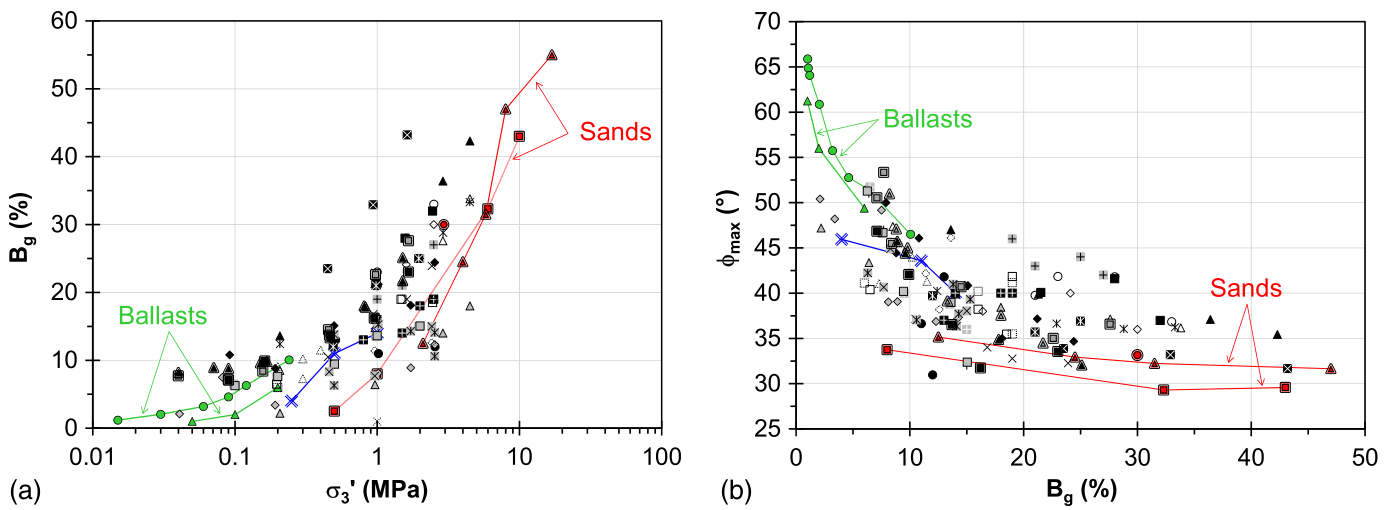
\includegraphics[width=0.8\textwidth]{figures/figure-3.png}
    \bicaption{Marsal’s breakage ratio}{Marsal破损率}
    \label{figure:3}
\end{figure}
    }

    \switchcolumn*

    It is well known that $B_g$ is expected to be inversely proportional to the initial uniformity coefficient $C_u=d_{60}/d_{10}$ \citep{Hardin19851177,Ovalle20162383}. However, it is not worth proposing a relationship for the current rockfill database given the large data scatter due to other independent variables that affect the material response.

    \switchcolumn

    众所周知,$B_g$与初始均匀系数$C_u=d_{60}/d_{10}$成反比\citep{Hardin19851177,Ovalle20162383}。然而,考虑到其他影响材料响应的自变量造成的大数据散点,对于目前的碎石数据库,提出一个关系是不值得的。

    \switchcolumn*[\biparagraph{Secant Young’s Modulus}{割线杨氏模量}]

    Young’s moduli values for rockfills have been proposed based on dam settlement analyses \citep{Hunter2003909,Kermani2018}. However, data from stress-controlled laboratory tests needed for calibration of constitutive models are scarce. Here, secant Young’s moduli from drained triaxial stress paths were obtained to compare the results with typical values used for sands. To avoid experimental scatter from data recorded at small strains in triaxial tests, a convenient modulus $E_{50}$ has been chosen, defined as the secant modulus associated with a deviatoric stress level ($q=\sigma_1^\prime-\sigma_3^\prime$) equal to half of the maximum strength. $E_{50}$ is commonly fitted by the following expression:

    \switchcolumn

    根据大坝沉降分析,提出了碎石料的杨氏模量值\citep{Hunter2003909,Kermani2018}。 但是,本构模型校准所需的应力控制实验室试验数据很少。 在这里,从排水的三轴应力路径获得了割线杨氏模量,将结果与用于砂土的典型值进行了比较。 为了避免在三轴试验中以小应变记录的数据产生实验性分散,我们选择了方便的模量$E_{50}$,定义为与偏应力水平($q=\sigma_1^\prime-\sigma_3^\prime$)相关联的正割模量,该水平等于最大强度的一半。$E_{50}$通常由以下表达式拟合:

    \CrossColumnText{
        \begin{align}
            E_{50}=K_{50} \cdot p_{a}\left(\frac{\sigma_{3}^{\prime}}{p_{a}}\right)^{n}
            \label{equation:3}
        \end{align}
    }

    \switchcolumn*

    \noindent
    where $n$ = fitted parameter, typically from 0.4 to 0.6 in sands \citep{Schanz1998383,Schanz1999281}; $K_{50}$ = reference normalized modulus; and $p_a=0.1$ MPa = reference pressure. \enautoref{figure:4} presents $E_{50}$ for all rockfill materials compared to data of dense quartzitic sands and ballasts. In addition, \enautoref{equation:1} is plotted assuming $n=0.5$ and typical values of $K_{50}$ of 200 and 400 for loose and dense sands, respectively \citep{Schanz1998383}. The comparison indicates that most rockfills have lower moduli than loose sands. By contrast, $E_{50}$ of ballasts at low pressure is similar to the values for dense sands, but tends to be in the range for rockfills at intermediate pressures of 100–200 kPa. As an explanation of this result, it is thought that even a small number of crushing events occurring in rockfill and ballast materials at relatively small strains (e.g., attrition process removing asperities) could result in a significant drop in material stiffness. At high stresses, crushing becomes significant in sands and the stiffness of sands and rockfills follows a similar trend.

    \switchcolumn

    \noindent
    其中$n$为拟合参数,通常在砂土中为0.4到0.6 \citep{Schanz1998383,Schanz1999281};$K_{50}$为参考归一化模量;$p_a=0.1$MPa为参考压力。 \cnautoref{figure:4}给出了所有碎石料的$E_{50}$与致密石英砂和石渣的数据的比较。 另外,\cnautoref{equation:1}的绘制假设$n=0.5$以及疏砂和密砂的$K_{50}$的典型值分别为200和400\citep{Schanz1998383}。 比较结果表明,大多数碎石料的模量均低于散砂。 相比之下,低压下的石渣的$E_{50}$与密砂的值相似,但在100-200kPa的中间压力下,往往处于碎石的范围内。 作为对这一结果的解释,人们认为,即使在相对较小的应变下在碎石和石渣材料中发生的少量压碎事件(例如,例如,摩擦过程消除磨损)也可能导致材料刚度的显着下降。 在高应力下,砂土的破碎变得很明显,砂土和碎石的硬度也遵循类似的趋势。

    \CrossColumnText{
        \sidebyside[verticalalignment=top][htb]{0.48\textwidth}{
    \begin{figure}[H]
        \centering
        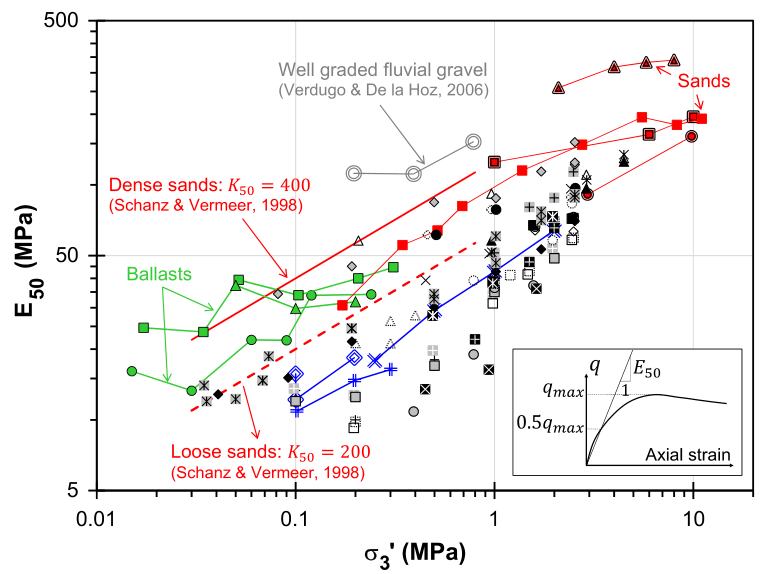
\includegraphics[width=\textwidth]{figures/figure-4.png}
        \bicaption{Secant Young’s modulus}{割线杨氏模量}
        \label{figure:4}
    \end{figure}
}{0.48\textwidth}{
    \begin{figure}[H]
        \centering
        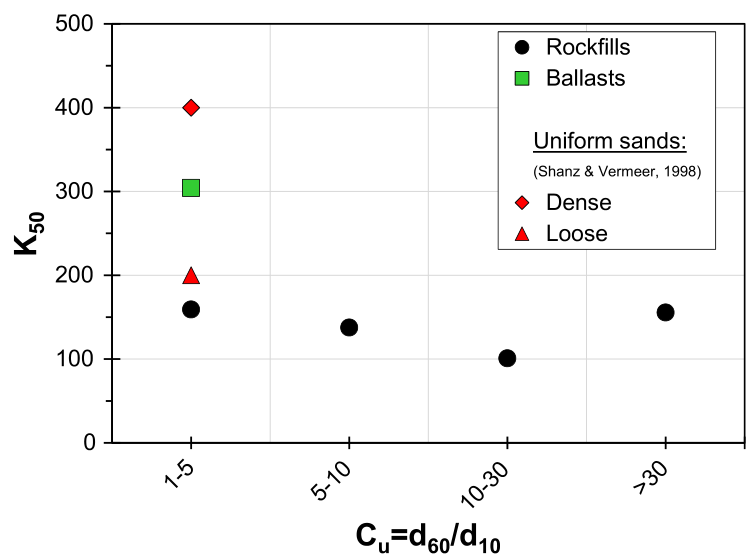
\includegraphics[width=\textwidth]{figures/figure-5.png}
        \bicaption{Normalized secant Young’s modulus}{归一化割线杨氏模量}
        \label{figure:5}
    \end{figure}
}
    }

    \switchcolumn*

    \enautoref{figure:4} also includes values of $E_{50}$ from drained triaxial tests on coarse, well-graded fluvial gravel composed of sound rounded clasts of $d_{\max}=200$ mm reported by \citet{DelaHozAlvarez2007} and \citet{Verdugo2007243}. In this case, the amount of particle crushing is considerably lower than in rockfills due to both high Cu and highly resistant rounded gravel clasts, resulting in $E_{50}$ being comparable to dense quartzitic sands.

    \switchcolumn

    \cnautoref{figure:4}还包含\citet{DelaHozAlvarez2007}以及\citet{Verdugo2007243}报道的对粗、级配良好的河流砾石进行的排水三轴试验的$E_{50}$值,这些砾石由$d_{\max}=200$毫米的良好圆形碎屑组成。 在这种情况下,由于高$C_u$和高强度的圆形砾石碎屑,颗粒破碎量要远低于碎石,使得$E_{50}$可与致密的石英砂媲美。

    \switchcolumn*

    For the data compiled here, $K_{50}$ from \enautoref{equation:3} was fitted by separating and averaging the data in ranges of initial $C_u$. As shown in \enautoref{figure:5}, regardless of the value of $C_u$, the data for rockfill are in a narrow band of $K_{50}=100–200$, typically associated with loose sands.

    \switchcolumn

    对于此处汇编的数据,请从\cnautoref{equation:3}中获取$K_{50}$。通过在初始$C_u$范围内分离和平均数据来拟合。 如\cnautoref{figure:5}所示,无论$C_u$的值如何,堆石的数据都在$K_{50}=100–200$的窄带中,通常与松散的砂土有关。
    
\end{ParaColumn}
\begin{ParaColumn}[\bisection*{Conclusions}{结论}]
    
    The compilation of large drained triaxial tests on coarse rockfill materials presented in this article includes samples with different relative densities, mineralogies, gradings, and particle shapes, resulting in significant data scatter. However, the minimum limit imposed on $d_{\max}$ reduces the potential for size effects, allowing an appropriate comparison with data on ballast and quartzitic dense sands, which are usually taken as a reference for mechanical parameters of granular materials.

    \switchcolumn

    本文介绍的对粗碎石材料进行的大排水三轴试验的汇编包括具有相对密度,矿物成分,级配等级和颗粒形状不同的样品,从而导致大量数据分散。 但是,对$d_{\max}$施加的最小的限制减小了尺寸影响的可能性,从而可以与石渣和石英质致密砂土的数据进行适当的比较,这些数据通常被用作颗粒材料力学参数的参考。
    
    \switchcolumn*

    The analyses show the typical behavior of crushable granular materials previously reported, namely, shear strength decreasing due to particle crushing when pressure increases. In this study, the magnitude of this phenomenon is highlighted in coarse, angular materials. In general, data on coarse rockfill materials confirm previously reported limits for average shear strength. Dense quartzitic sands reasonably correspond to the range of average to low shear strength values for rockfills in a large range from low to high pressure. At low pressure of $\sigma_n^\prime<0.2$ MPa, where the amount of crushing is still not significant, rockfills and ballasts have consistently higher shear strength than dense quartzitic sands, and the maximum internal friction angle is higher than 45°. At high pressure, the amount of grain breakage increases and the maximum internal friction angle of sands and rockfills is between 30° and 40°. According to the analysis, previous limits for low shear strength proposed in the literature seem conservative at low stresses. A new expression is provided in this paper that considers higher strength at normal stress lower than 0.7 MPa.

    \switchcolumn

    分析显示了先前报道的可破碎粒状材料的典型行为,即当压力增加时,由于颗粒破碎,抗剪强度降低。在本研究中,这种现象的量级在粗糙、有角的材料中得到了突出。一般来说,粗石料的数据证实了先前报告的平均抗剪强度极限。致密石英岩砂合理地对应于低压力到高压力大范围内的平均到低抗剪强度的范围。在低压$\sigma_n^\prime<0.2$MPa时,破碎量仍然不显著的情况下,碎石和石渣的抗剪强度始终高于致密石英砂,最大内摩擦角大于45°。在高压下,颗粒破碎量增大,砂土与碎石的最大内摩擦角在30°到40°之间。根据分析,以往文献中提出的低抗剪强度限值在低应力下显得保守。本文提出了一种考虑高强度时法向应力小于0.7MPa的新表达式。

    \switchcolumn*

    In general, dense quartzitic sands are stiffer than rockfills at low stresses and their secant Young’s moduli tends to have similar values at high stresses, probably due to the significant amount of particle crushing in both materials. Normalized Young’s moduli at reference pressures for rockfills are in the same typical range for loose sands.

    \switchcolumn

    通常,致密的石英砂在低应力下比碎石坚硬,其割线杨氏模量在高应力下往往具有相似的值,这可能是由于两种材料中大量的颗粒被压碎造成的。 对于松散砂体,参考压力下的归一化杨氏模量在相同的典型范围内。

\end{ParaColumn}
\begin{ParaColumn}[\bisection*{Data Availability Statement}{数据可用性声明}]

    Compiled and new data on rockfill materials supporting this paper are available at \href{https://doi.org/10.5281/zenodo.3625778}{here}.

    \switchcolumn

    支持该论文的碎石的汇编数据和新数据可以在\href{https://doi.org/10.5281/zenodo.3625778}{这里}找到。

    \switchcolumn*[\bisection*{Acknowledgments}{致谢}]

    The authors gratefully acknowledge Fortescue Metals Group Ltd (Australia), Conseil Général du Gard (France), and Ecole Centrale of Lyon (leader of French ANR PEDRA project) for permission to publish the results of testing on rockfill materials. The first author acknowledges the support of the Natural Sciences and Engineering Research Council of Canada (NSERC) [funding reference number RGPIN-2019-06118]. The second author acknowledges the support of SRK Consulting (Australasia) Pty Ltd and the University of Newcastle (Australia).

    \switchcolumn

    作者非常感谢Fortescue Metals Group Ltd (Australia),ConseilGénéraldu Gard (France)和Ecole Centrale of Lyon(French ANR PEDRA项目的负责人)获准发表关于碎石料的试验结果。 第一作者感谢加拿大自然科学与工程研究委员会(NSERC)的支持[资金参考号RGPIN-2019-06118]。 第二作者感谢SRK Consulting(Australasia)Pty Ltd和University of Newcastle(Australia)的支持。

\end{ParaColumn}

\bibliographystyle{plainnat}
\bibliography{Ovalle2020.bib}
    
\end{document}